\documentclass[runningheads]{llncs}
\usepackage[T1]{fontenc}
\usepackage{lmodern}
\usepackage{graphicx}
\usepackage{amsmath,amssymb}
\usepackage{booktabs}
\usepackage{array}
\usepackage{microtype}
\usepackage{xcolor}
\usepackage[hidelinks]{hyperref}
\newcommand{\R}{\mathbb{R}}
\newcommand{\B}{\mathcal{B}}
\newcommand{\deltab}{\delta}
\renewcommand{\paragraph}[1]{\smallskip\noindent\textbf{#1}\ }

\begin{document}
\title{TRIAD: Bundle Completion from Shared Relations Instead of Item Embeddings}
\titlerunning{TRIAD: Bundle Completion from Shared Relations}
\author{Anonymous Submission}
\authorrunning{Anonymous}
\institute{Anonymous Institution}
\maketitle

% =====================================================================================================================
\begin{abstract}
Bundle completion asks a system to fill in the missing items of a partial bundle, such as an outfit or a playlist.
Current neural models learn an embedding for every item from the few bundles that contain it, so their size grows
with the catalogue and rarely bundled items are poorly described. We start from the observation that what makes items
go together is mostly shared across items: which categories or artists appear together, how similar two items are,
and how often they have been bundled. We propose TRIAD, a model whose 41,368 parameters describe such relations and
never a single item. TRIAD scores a candidate by a query-dependent weighted sum of three relations to the seeds:
content similarity, a shared-label score whose sign is learned, and discounted co-occurrence counts. It is trained without leakage: each training bundle is scored with its own contribution removed from every
statistic. On seven datasets from fashion, music and e-commerce, we rerun two recent neural models on identical splits
and features and tune thirteen simple baselines, giving the five main ones the same frequency prior that TRIAD
learns. TRIAD ranks the missing items better than every rerun neural model. Under the ten-candidate protocol of
Bundle-MLLM, which fine-tunes a 7B-parameter language model, TRIAD also scores above Bundle-MLLM's published
HitRate@1 on all four datasets it reports. Against the best simple baseline it is
ahead on outfits and playlists (+.007 to +.048 NDCG@20, Holm-corrected paired tests) and level on three
e-commerce datasets of short bundles, where most of its apparent lead comes from ranking items that occur in no
training bundle above items seen once; adding never-bundled items to the catalogue removes that gain. Trained on fewer bundles,
TRIAD keeps its lead on playlists down to 50 bundles and on outfits down to 1\% of POG\_DENSE, but falls behind on
e-commerce with 100 or fewer.
\keywords{bundle completion \and bundle construction \and recommender systems \and label relations}
\end{abstract}

% =====================================================================================================================
\section{Introduction}

A bundle is a set of items that are used together: an outfit of a top, trousers and shoes; a playlist built around a
few artists; a set of computer parts. Platforms rarely build bundles from nothing. A merchandiser picks one or two
products, or a listener adds a few songs, and the system is asked to suggest the rest. This is \emph{bundle
completion}: given some items of a bundle (the \emph{seeds}), rank the whole catalogue so that the missing items come
first (Fig.~\ref{fig:intro}a) \cite{clhe,ramen}. The task differs from user-based recommendation, because the query
is a set of items, not a user, and the answer must fit the seeds as a group.

Recent models treat bundle completion as representation learning. CLHE \cite{clhe} describes every item by an ID
embedding, multimodal features and a graph embedding, fuses them with self-attention, pools the seeds with a second
attention layer, and trains with reconstruction and contrastive losses. RaMen \cite{ramen} adds attention over an
item--item graph and a hypergraph of latent intents. Both score a candidate by an inner product between a bundle
vector and the candidate's item vector, and both learn part of that item vector from the bundles the item appears in.
Bundle-MLLM \cite{bundlemllm} goes further and fine-tunes a 7B-parameter language model to pick the missing item from
ten candidates.

This design ties what the model knows to individual items (Fig.~\ref{fig:intro}b). On our datasets CLHE has 3.7\,M
to 29\,M trained parameters and RaMen 1.3\,M to 67\,M, on large catalogues mostly rows of per-item tables. Each row is fitted only from
the bundles that contain its item, and bundle data are long-tailed: most items appear in a handful of bundles, and new
items in none. Bundle-MLLM runs a 6.7B-parameter model, with about 4\,M LoRA weights trained on top, for every
question. Large models are also hard to fit from such data, and their gains over well-tuned simple methods
should be checked, not assumed \cite{dacrema}.

Much of what makes items go together is not specific to an item. An outfit takes one item from each of several
categories and seldom two from the same one. A playlist does the opposite and returns to the same artists. Which label
goes with which is a relation among a few hundred labels, so every training bundle helps to learn it. Content
similarity and co-occurrence counts are also functions of item pairs that can be scored the same way for all items.
How much each kind of evidence should count depends on the query: a seed that occurs in many training bundles has
reliable co-occurrence counts, and a seed that occurs in none has only its content and its labels.

We build on this observation with \textbf{TRIAD}, named after its three relations between the seeds and a candidate.
TRIAD scores a candidate by a gated sum of three kinds of evidence: content, labels and co-occurrence
(Fig.~\ref{fig:intro}c). Its 41,368 parameters describe these relations, and none belongs to an item, so an item that
never appeared in a training bundle is scored by the same function as any other. Our contributions are:
\begin{itemize}
\item \textbf{A model with no per-item parameters.} Each term is a small function of statistics shared by all items:
a bilinear map of item features and partner histories, a same-label score whose sign is learned per domain, and
degree-discounted co-occurrence counts with learned exponents. Training removes each bundle's own contribution from
every count, so the model never sees statistics that contain the answer.
\item \textbf{A matched comparison.} We rerun CLHE and RaMen as released by their authors, on identical splits and with
identical item features, with graphs built from training bundles only, and compare against thirteen tuned simple baselines,
four of which use the same labels as TRIAD. Because the released catalogues list the items of every split, we also
give the simple baselines the frequency prior that TRIAD learns, and report TRIAD without it. TRIAD is ahead of every
rerun neural model, ahead of the best simple baseline on outfits and playlists, and level with it on short
e-commerce bundles. Scored without retraining under the sampled protocols of Bundle-MLLM and DDBC, TRIAD is also
above their numbers.
\item \textbf{Guidance on when a learned model pays off.} By training on subsets from 50 bundles up to the full training set, against
simple baselines that also get the prior, we show that TRIAD leads from 50 playlists and from 1\% of the POG\_DENSE
outfits, but on short e-commerce bundles is never significantly ahead and falls behind a tuned label, neighbourhood and content
scorer with 100 or fewer; the cause is overfitting rather than too few training steps. We also show that the
unseen-item bonus is learned from training data alone and follows the catalogue: with never-bundled items added it
turns into a penalty and its gain disappears.
\end{itemize}

\begin{figure}[t]
\centering
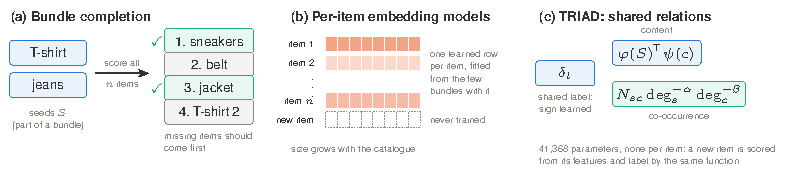
\includegraphics[width=\textwidth]{figs/fig1.pdf}
\caption{(a) Bundle completion ranks every catalogue item for a partial bundle. (b) Per-item models such as CLHE and
RaMen store part of their knowledge in one learned row per item. (c) TRIAD learns relations that are shared by all
items: over labels, between item features, and over co-occurrence counts.}
\label{fig:intro}
\end{figure}

% =====================================================================================================================
\section{Related Work}

\paragraph{Bundle construction and completion.} Bundle recommendation ranks existing bundles for a user
\cite{bgcn,crosscbr}, and personalized bundle generation creates a bundle for a user \cite{bgn,pog}. Bundle
construction, the setting of this paper, starts from a partial bundle and has no user. CLHE \cite{clhe} and RaMen
\cite{ramen} learn item representations from several views and score candidates against a pooled seed vector.
Bundle-MLLM \cite{bundlemllm} fine-tunes a multimodal language model to pick the next item from a short candidate list,
and DDBC \cite{ddbc} generates bundles with discrete diffusion over item codes. Large language models have also been
prompted to generate bundles from sessions \cite{adabundle}, and Caro \cite{caro} refines CLHE-style item
representations with category-wise and cross-modal learning. Most of these models learn a representation per item. TRIAD learns none, and we compare against CLHE and RaMen directly.

\paragraph{Set and basket completion.} Bundle completion scores a set, so it relates to permutation-invariant set
models such as DeepSets \cite{deepsets} and the Set Transformer \cite{settransformer}, and to basket completion with
determinantal point processes \cite{gartrell2017}. These models learn item embeddings and pool them; TRIAD instead
pools fixed statistics (mean features, label counts, co-occurrence counts) and learns only how to weigh them.
Playlist continuation, studied at scale in the RecSys Challenge 2018 \cite{spotify}, was won by a two-stage system of
matrix factorization retrieval and re-ranking \cite{volkovs2018}; we use the same Spotify data through CLHE's splits.

\paragraph{Items without interactions.} Feature-based models such as LightFM \cite{lightfm} and DropoutNet
\cite{dropoutnet} score items with no interactions by mapping their features into the latent space of the
interaction model. TRIAD has no per-item latent space, so a new item is scored by the same content and label terms as
any other, and the gate shifts weight to them when the seeds themselves are unseen.

\paragraph{Compatibility and complementarity.} Fashion compatibility models learn which items fit together, for
example from images \cite{han2017}, with separate spaces per category pair \cite{vasileva2018}, or as complements in
product graphs \cite{mcauley}. These works show that the relation between two items depends on their categories.
TRIAD keeps one label-level rule, whether a shared label helps or hurts, which differs by domain
(Section~\ref{sec:learned}), and leaves which different labels go together to the item-level co-occurrence counts.

\paragraph{Simple item-to-item methods.} Neighbourhood methods such as ItemKNN \cite{sarwar2001} and RP3$\beta$
\cite{rp3beta}, the linear model EASE \cite{steck2019} and graph filters such as GF-CF \cite{gfcf} and SGFCF
\cite{sgfcf} remain strong in recommendation, and several neural models have been found to trail them once they are
tuned \cite{dacrema,rendle2020}. Latent-factor and graph models \cite{hu2008,bpr,lightgcn} learn one embedding per
item; iALS \cite{hu2008} represents this family among our baselines. RP3$\beta$ and the graph filters divide co-occurrence by item degree raised to a
tuned power; TRIAD learns these powers. We tune these methods on validation and add label-aware variants, so that a
gain of TRIAD cannot come from labels alone.

\paragraph{Leakage in training statistics.} When a model is trained on statistics computed from the same examples
it is trained on, each example sees a version of its own answer \cite{kapoor2023}. TRIAD removes each training
bundle from its own counts exactly.

% =====================================================================================================================
\section{Method}
\label{sec:method}

\subsection{Task and notation}

The catalogue has $n$ items. Item $c$ has a feature vector $x_c\in\R^{d}$ ($X\in\R^{n\times d}$, rows normalized to
unit length) and, at each label level $l$, a label $g_l(c)$; the levels are the category for fashion and e-commerce,
and artist and album for music. From the training bundles $\B$ we count $N_{sc}$, the number of bundles that contain
both $s$ and $c$ ($s\neq c$), the item frequency $f_c$ (bundles that contain $c$) and the degree
$\deg_c=\sum_s N_{sc}$. A query is a seed set $S$, part of an unseen bundle; the task is to rank all items not in
$S$ so that the rest of the bundle comes first.

\subsection{Item features and labels}
\label{sec:features}

Every method that uses item features or labels receives the same ones, described below. TRIAD then projects the
features to $d=128$ (last paragraph).

\paragraph{POG and POG\_DENSE.} The item features released with CLHE \cite{clhe}: a BLIP \cite{blip} image
embedding and a BLIP text embedding of the item description, 768 dimensions each. Label: the item's category (67 and 72 values).

\paragraph{Spotify and Spotify\_sparse.} The released CLAP \cite{clap} audio embedding of the track and CLAP text
embedding of its metadata, 512 dimensions each. Labels at two levels: artist and album.

\paragraph{Electronic, Food and Clothing.} No features are released, and only Electronic lists image links (451 of
3,499 items; those we tried do not resolve). We embed each item title, which every item has, with the text encoder of
BLIP (the base image--text matching model fine-tuned on COCO, titles truncated to 128 tokens) and take the
768-dimensional [CLS] vector, so these datasets have one modality, text. Label: the item's category string as released, that is, all of its
category paths together (479, 836 and 2,033 values).

\paragraph{Projection.} Let $X_1\in\R^{n\times d_1}$ and $X_2\in\R^{n\times d_2}$ be the two modalities (one on
e-commerce). Each is row-normalized, $\hat X_k=\mathrm{diag}(\lVert X_k\rVert_{\mathrm{row}})^{-1}X_k$, the two are
concatenated, $\tilde X=[\hat X_1\ \hat X_2]$, and rows are normalized again so that both modalities count equally. A
rank-128 truncated SVD $\tilde X\approx U_{128}\Sigma_{128}V_{128}^{\top}$ (randomized, fixed seed) gives
$X=U_{128}\Sigma_{128}\in\R^{n\times128}$, the coordinates of each item along the 128 leading directions; its rows are
normalized to unit length. The projection uses no bundle and no label. The simple content baselines use this same
$X$; CLHE and RaMen take the full, unprojected vectors, as they were designed to. For every number we report we
verified that the POG and Spotify feature files are byte-identical to the public release that CLHE and RaMen use,
that every simple baseline (all datasets, all training-set sizes) uses exactly TRIAD's matrix $X$, and that the
e-commerce vectors given to CLHE and RaMen are the BLIP title vectors that TRIAD projects. DDBC is rerun from its
released checkpoints with its own released inputs, and Bundle-MLLM's numbers are the published ones.

\subsection{Overview}

TRIAD gives every item $c$ the score
\begin{equation}
s(c\mid S)=w_C(S)\,C(S,c)+\textstyle\sum_l w_l(S)\,L_l(S,c)+w_G(S)\,G(S,c),
\label{eq:score}
\end{equation}
the sum of a content term $C$, one label term $L_l$ per level and a graph term $G$, weighted by a gate $w(S)$ that
depends on the query (Fig.~\ref{fig:arch}). Each term answers one question about the candidate: does it look like it
belongs with the seeds, does it share a label with a seed, and has it been bundled with the seeds before? The
three answers are useful at different times, which is why their weights depend on the query.

\begin{figure}[t]
\centering
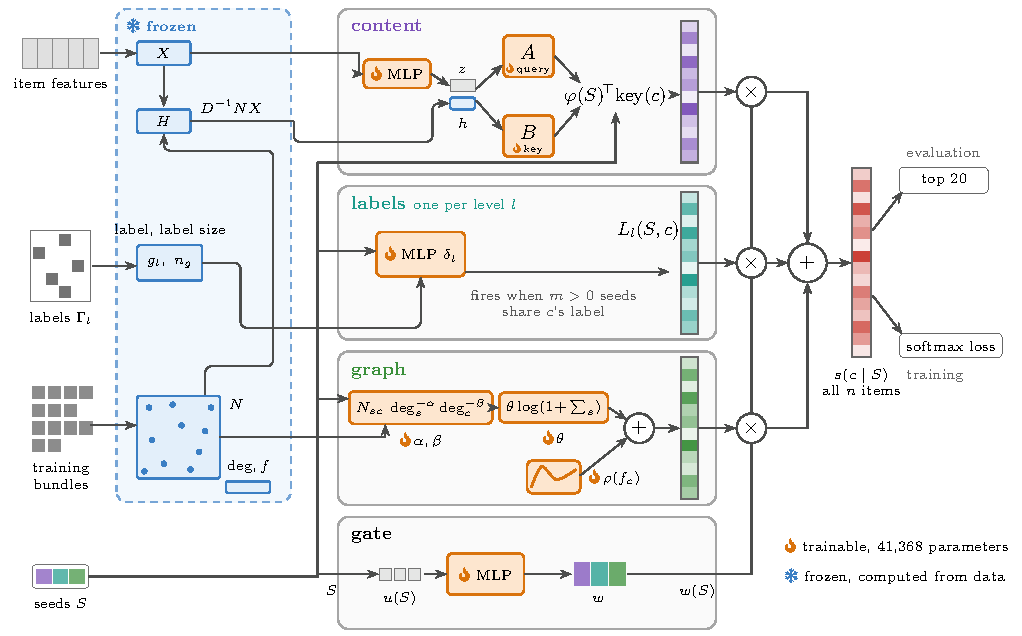
\includegraphics[width=\textwidth]{figs/fig2_arch.pdf}
\caption{TRIAD. Frozen structures (blue) are computed once from the item features, labels and training bundles.
Each term (content, labels, graph) gives a score vector over all $n$ items; the gate weights them per query, and their
sum ranks the catalogue. All 41,368 trained parameters (orange) are shared by all items.}
\label{fig:arch}
\end{figure}

\subsection{Content}

The content term compares the seeds with the candidate through learned rank-64 maps. Item features are first refined
by a small residual network, $Z=\mathrm{normalize}(X+\mathrm{MLP}(X))$. Each item also gets a \emph{partner history}
$h_c$, the count-weighted mean feature of the items it has been bundled with: $H=\mathrm{diag}(\deg)^{-1}NX$. The
history describes an item by what it has been bundled with, not only by what it is. Then
\begin{equation}
C(S,c)=\varphi(S)^{\top}\psi(c),\ \ \varphi(S)=\tfrac{1}{|S|}\textstyle\sum_{s\in S}(A_z z_s+A_h h_s),\ \
\psi(c)=B_z z_c+B_h h_c
\end{equation}
with $A_z,A_h,B_z,B_h\in\R^{64\times d}$. Separate seed-side ($A$) and candidate-side ($B$) maps let the score be
asymmetric: a jacket can call for boots without boots calling for a jacket. The maps start at a scaled identity on
the first 64 feature coordinates, so training starts from plain feature similarity.

\subsection{Labels}

Let $m=t_{g(c)}(S)$ be the number of seeds that share the candidate's label at level $l$, and $n_g$ the number of
items with label $g$. The label term scores a shared label,
\begin{equation}
L_l(S,c)=\deltab_l\big(\log(1+m),\log|S|,\log(1+n_{g(c)})\big)\cdot[m>0],
\end{equation}
where $\deltab_l$ is an MLP with 16 hidden units shared by all labels of the level. Its output can be negative, so the
model can learn that sharing a label is evidence against a candidate, as in an outfit, which takes one item per
category. Sharing a small label is a strong hint, while sharing a large one (``shoes'') says little, which is why
$n_g$ is an input. The term reads only labels, so an item never seen in training is scored through its label like any
other. Which \emph{different} labels go together, such as skirts with sandals, is not a separate term: the item-level
counts $N$ already hold it, and a label-level table $\Gamma^{\top}N\Gamma$ would only be a coarser summary of them
(Section~\ref{sec:ablation}).

\subsection{Graph}

The graph term uses direct co-occurrence with the seeds, discounted for items that are bundled with everything:
\begin{equation}
G(S,c)=\theta\log\Big(1+\textstyle\sum_{s\in S}N_{sc}\deg_s^{-\alpha}\deg_c^{-\beta}\Big)+\rho\big(\log(1+f_c)\big),
\end{equation}
with learned $\theta,\alpha,\beta$ and a small MLP $\rho$ that learns a popularity prior. Only the stored non-zero
counts of the seeds' rows are read, so the cost per query is the number of the seeds' partners, not $n$.

\subsection{Gate}

The gate reads three statistics of the query: its size $\log|S|$, the mean seed frequency
$\tfrac{1}{|S|}\sum_{s\in S}\log(1+f_s)$ and the share of seeds with $f_s=0$. From these $u(S)$ it returns the weights $w(S)=\mathrm{softplus}(\mathrm{MLP}(u(S)))$, one per term. A query
whose seeds were never bundled has no co-occurrence evidence, and the gate can move weight to content and labels.

\subsection{Training without leakage}

\paragraph{Examples and loss.} Each step takes 32 training bundles and hides a random part of each: half of the items
with probability $1/2$, otherwise a uniform cut, so that queries of all sizes are seen. The visible items are the
seeds. Each hidden item $j$ competes with all catalogue items outside its bundle through the loss
$\mathrm{softplus}(\mathrm{LSE}_{c\notin b}\,s(c\mid S)-s(j\mid S))$, averaged over hidden items.

\paragraph{Leave-one-out statistics.} A training bundle $b$ is part of $N$, $f$, $\deg$ and $H$. If it stayed there,
the counts between its seeds and its hidden items would contain the answer, and the model would learn to trust
co-occurrence far more than it should at test time, where no such count exists. So each training bundle is scored
with its own contribution removed: $N_{sc}-1$ for pairs inside $b$, $\deg-(|b|-1)$ and $f-1$ for its members, and
the same correction in $H$. Only the counts of the seeds' rows are touched, so the correction is cheap.
The label term reads no counts, so it needs no correction.

\paragraph{One configuration.} Content rank 64, AdamW \cite{adamw} with learning rate $10^{-2}$ for the small
relation parameters ($\deltab_l$, $\alpha$, $\beta$, $\theta$, $\rho$, gate) and $10^{-3}$ for the content maps and
the feature encoder, weight decay $10^{-3}$, gradients clipped at norm 5, early stopping on validation NDCG@20 with
patience 6 and at most 100 epochs; the parameters of the best epoch are kept. Every small network ($\deltab_l$, $\rho$,
gate, encoder) has one GELU hidden layer. At initialization the encoder's last layer is zero ($Z=X$), the content maps
are $\sqrt{10}\,[I_{64}\ 0]$ for $A_z,B_z$ and zero for $A_h,B_h$, $\alpha=\beta=0$, $\theta=1$, and the gate's last layer
has zero weights and bias $\log(e-1)$, so every term starts with weight 1; $\deltab_l$ and $\rho$ start from the standard
uniform initialization scaled by fan-in. Nothing is tuned per dataset, and the e-commerce datasets were not used while
the model was developed. The model has 41,368 parameters, 41,466 with two label levels, independent of $n$
(Table~\ref{tab:params}).

\begin{table}[t]
\centering
\caption{Trained parameters of TRIAD ($d=128$, rank 64). None of them belongs to an item or a label; the frozen
structures grow with the catalogue but are rebuilt from the data and not trained.}
\label{tab:params}
\setlength{\tabcolsep}{4pt}
\small
\begin{tabular}{llr}
\toprule
Component & Shape & Parameters\\
\midrule
Content maps $A_z,B_z,A_h,B_h$ & $4\times(64\times128)$ & 32,768\\
Feature encoder (residual MLP) & $128\to32\to128$ & 8,352\\
Same-label score $\deltab_l$ & $3\to16\to1$ per level & 81 per level\\
Degree exponents $\alpha,\beta$ and scale $\theta$ & & 3\\
Popularity prior $\rho$ & $1\to16\to1$ & 49\\
Gate & $3\to16\to(2+\text{levels})$ & 115 / 132\\
\midrule
Total & & 41,368 / 41,466\\
Frozen: $X$, $N$, $\deg$, $f$, $H$, labels & grow with $n$ & not trained\\
\bottomrule
\end{tabular}
\end{table}

\paragraph{Cost.} Setup computes the pair counts ($\sum_b|b|^2$ over training bundles), degrees, frequencies and
partner histories once. Per query, the graph term reads $\sum_{s\in S}\deg_s$ stored counts, the content term is one
$64\times n$ product and the label term one lookup per item and level. Training one seed takes seconds on
e-commerce, about an hour on POG and a few hours on Spotify on one CPU thread.

% =====================================================================================================================
\section{Experiments}

We ask four questions. Does TRIAD rank the missing items better than neural and simple baselines under one protocol
(Section~\ref{sec:main})? Which parts matter (Section~\ref{sec:ablation})? How much training data does it need
(Section~\ref{sec:budget})? And what does it learn (Section~\ref{sec:learned})?

\subsection{Setup}

\paragraph{Datasets.} We use the seven public datasets that come with real bundles (Table~\ref{tab:data}). POG and
POG\_DENSE are outfits made by Taobao's fashion experts for Alibaba iFashion \cite{pog}, and Spotify and
Spotify\_sparse are playlists made by Spotify users, from the RecSys Challenge 2018 \cite{spotify}, all with the train, validation and test files released with CLHE \cite{clhe}, used
unchanged. Each test bundle comes split into seeds and held-out items. Electronic, Food and Clothing are product
bundles released by Sun et al.\ \cite{bundlerec}, marked by crowd workers in Amazon shopping sessions, each with a
stated purpose; we count repeated items inside a bundle once, remove duplicate bundles and
bundles with fewer than two distinct items, split the rest 70/10/20 with a fixed seed and hide half of each validation
and test bundle. Item features and labels are described in
Section~\ref{sec:features}.

\begin{table}[t]
\centering
\caption{Datasets. Size: mean items per training bundle. Labels: values per level (category; artist, album).
Test: test queries, with clean ones in brackets when some test bundles also occur in training or validation.}
\label{tab:data}
\setlength{\tabcolsep}{3pt}
\small
\begin{tabular}{llrrrrl}
\toprule
Domain & Dataset & Items & Train & Size & Test & Labels\\
\midrule
E-commerce & Electronic & 3,499 & 1,211 & 3.5 & 346 & 479\\
 & Food & 3,767 & 1,232 & 3.5 & 353 & 836\\
 & Clothing & 4,487 & 1,294 & 3.3 & 371 & 2,033\\
Fashion & POG\_DENSE & 31,217 & 20,780 & 3.6 & 5,938 (5,547) & 67\\
 & POG & 48,676 & 14,000 & 3.6 & 4,000 (3,995) & 72\\
Music & Spotify\_sparse & 213,325 & 8,740 & 44.2 & 2,498 (2,497) & 43,039; 98,674\\
 & Spotify & 254,155 & 14,000 & 63.6 & 4,000 (3,995) & 49,164; 116,217\\
\bottomrule
\end{tabular}
\end{table}

\paragraph{Protocol.} Every method ranks the full catalogue with the seeds removed, and we report Recall@20 and
NDCG@20. With $T$ the held-out items and $\mathrm{hit}_k=1$ if the $k$-th ranked item is in $T$,
$\mathrm{Recall@20}=\frac{1}{|T|}\sum_{k\le20}\mathrm{hit}_k$ and
$\mathrm{NDCG@20}=\sum_{k\le20}\frac{\mathrm{hit}_k}{\log_2(k+1)}\big/\sum_{k\le\min(|T|,20)}\frac{1}{\log_2(k+1)}$;
exact ties go to the lower item ID, so results do not depend on batching. Some released test bundles of POG and Spotify also occur, complete, in the training or validation files; a
method that memorizes bundles gets them for free, so we report \emph{clean} test queries, which exclude them
(Table~\ref{tab:data}). Learned models are run with seeds 0, 1 and 2, and per-query metrics are averaged over seeds.
Differences come with a 95\% paired bootstrap interval and a paired sign-flip test, both resampling clusters of
identical bundles \cite{efron1993,smucker2007}, with Holm's correction \cite{holm1979} within each table. Ranking
the full catalogue avoids the bias of sampled metrics \cite{krichene2020}.

\paragraph{Baselines.} \emph{Simple:} popularity, co-occurrence, ItemKNN \cite{sarwar2001}, RP3$\beta$
\cite{rp3beta}, EASE \cite{steck2019}, GF-CF \cite{gfcf}, SGFCF \cite{sgfcf}, iALS \cite{hu2008}, a blend of ItemKNN
with content cosine, and four label-aware methods that use TRIAD's labels: same-label counts, label transition
probabilities, and the better of the two blended with ItemKNN, with and without content (EASE is too large for
Spotify). Every method is tuned on validation NDCG@20, and the best one per dataset is chosen on validation as well.
The five main ones (ItemKNN, RP3$\beta$, EASE, content+ItemKNN, label+ItemKNN+content) are also given the same
frequency prior that TRIAD learns (Section~\ref{sec:fair}), with its weight chosen on validation. \emph{Neural:} CLHE \cite{clhe} and RaMen \cite{ramen},
rerun as released by their authors, with settings chosen on validation. Both use the same item features as TRIAD. Their user or
item graphs are built from training bundles only, the information TRIAD has. RaMen's release does not include the construction of its
item--item graph, so we built it as its paper describes. On full Spotify, CLHE ran at batch size 128 instead of 256 to fit in GPU
memory, and only one of three seeds finished within the 12-hour limit, so it is not tested there. We did not rerun
RaMen on POG and Spotify and quote its published numbers, which use the same split files. Table~\ref{tab:tuning}
lists what each method tunes: every baseline with settings gets a validation grid, while TRIAD uses one configuration everywhere.

\begin{table}[t]
\centering
\caption{Tuning effort. Every setting is chosen on validation NDCG@20 and test is scored once. Settings: number of
configurations tried per dataset. Blends keep the setting already chosen for ItemKNN (and for the label method). With
two label levels (music) the label methods also try five level weightings.}
\label{tab:tuning}
\setlength{\tabcolsep}{3pt}
\scriptsize
\begin{tabular}{l>{\raggedright\arraybackslash}p{.54\textwidth}r}
\toprule
Method & Values tried & Settings\\
\midrule
Popularity, co-occurrence & none & 1\\
ItemKNN & neighbours $\{50,200,1000\}\times$ shrinkage $\{0,10,100\}$ & 9\\
RP3$\beta$ & $\alpha\in\{.5,1\}\times\beta\in\{0,.25,.5,.75\}$ & 8\\
EASE & L2 $\in\{50,200,500,1000,3000\}$ & 5\\
GF-CF & rank $\{64,256\}\times$ ideal-filter weight $\{0,.1,.3,1,3\}$ & 10\\
SGFCF & rank $\{64,256\}\times\epsilon\{.3,.5\}\times\beta\{1,2.5\}\times\gamma\{0,.5,1\}$ & 24\\
iALS & rank $\{64,128\}\times\alpha\{5,20\}\times$ L2 $\{1,10\}$ & 8\\
Content+ItemKNN & content weight $\{0,.1,.2,.3,.5,.7,.9,1\}$ & 8\\
Same label & popularity weight $\{0,.1,.3,1\}$ & 4 / 20\\
Label transition & popularity weight $\{0,.5,1,2\}\times$ smoothing $\{10^{-4},10^{-2}\}$ & 8 / 40\\
Label+ItemKNN & the better label method; label weight $\{0,.1,.2,.3,.5,.7,.9,1\}$ & 8\\
Label+ItemKNN+content & content weight $\{0,.05,.1,.2,.3,.5\}$ & 6\\
+ frequency prior (five main) & $\lambda\in\{0,.01,.03,.1,.3,1,3\}$, jointly with the blends' mixing weight (8 or 11 values) & 7--77\\
\midrule
CLHE & POG, Spotify: the authors' setting for that dataset; e-commerce: the best on validation of the four released
settings (one seed), then three seeds & 1 / 4\\
RaMen & e-commerce: learning rate $10^{-3}$, GAT layers $\{2,4\}\times\gamma\{.1,.3,.5,.7,.9\}$ (one seed), then three
seeds; POG, Spotify: published & 10\\
\midrule
TRIAD & one configuration for all datasets (Section~\ref{sec:method}); only the epoch is chosen on validation & 1\\
\bottomrule
\end{tabular}
\end{table}

\subsection{Equal information: the catalogue and unseen items}
\label{sec:fair}

Every method receives the same catalogue: the $n$ items with their features and labels, as released with the data
and as CLHE and RaMen also use it. On all seven datasets this catalogue is exactly the set of items that occur in some
training, validation or test bundle, so the 19--25\% of items that occur in no training
bundle ($f=0$) are all items of validation or test bundles. The catalogue reveals that these items exist, with their
features and labels, but not which bundles hold them; the co-occurrence counts come from training bundles only. Such
items are likely targets: 41--67\% of the e-commerce test targets, 23\% on POG\_DENSE, 59\% on POG, 29\% on
Spotify\_sparse and 14\% on Spotify have $f=0$.

TRIAD learns this from its training loss. Under leave-one-out, a training target that occurs in no other training
bundle has $f=0$, and it competes in the full-catalogue softmax with the other $f=0$ items, which are the
validation- and test-only items. Measured on training bundles in this way, the base-rate gap between $f=0$ and $f=1$
is 1.3--2.2, within .25 of the gap on test on every dataset, because bundle data are long-tailed (14--64\% of training
targets occur in no other training bundle). The learned bonus $w_G(\rho(0)-\rho(\log 2))$ on Electronic is already
2.0 after the first epoch and stays between 1.2 and 2.0 over 30 epochs without early stopping, so it comes from
training, not from choosing the epoch on validation. Frequency-based baselines, in contrast, rank $f=0$ items last, the popularity bias that recommenders usually
have \cite{abdollahpouri2017}.
No test answer is used, but the bonus pays off only because the catalogue holds no items outside the bundles; in a
store catalogue with many never-bundled items it would be spread over many non-targets. We therefore make the
comparison fair in two directions.

\paragraph{Simple baselines get the same prior.} For each of the five main simple baselines we add
$\lambda\,b(f_c)$ to its per-query max-scaled score, where $b$ is the base rate of validation targets by training
frequency (the bins of Section~\ref{sec:learned}, add-one smoothed), and choose $\lambda\in\{0,.01,.03,.1,.3,1,3\}$
on validation NDCG@20 together with the blends' mixing weight. With $\lambda=0$ every baseline number reported without the
prior is reproduced to within $10^{-6}$. The prior helps the content blends most on e-commerce (Clothing .359 $\to$ .427 NDCG@20 for
content+ItemKNN, Food .445 $\to$ .460, Electronic .302 $\to$ .312), and helps little on POG and Spotify, where the
baseline chosen on validation does not use it on three of the four datasets.

\paragraph{TRIAD without the unseen-item bonus.} At test time we replace $\rho$ of every item with $f=0$ by its value
at $f=1$. This costs TRIAD .028, .029 and .084 NDCG@20 on Electronic, Food and Clothing, .002 on POG, .001 on
Spotify\_sparse and nothing on POG\_DENSE and Spotify. All results below use the simple baselines with the prior,
and Tables~\ref{tab:main} and~\ref{tab:tests} also report TRIAD without the bonus.

\paragraph{The bonus follows the catalogue, not the split.} We test both claims, that the bonus is learned
from training data alone and that its payoff depends on the catalogue, on Electronic and Food (Table~\ref{tab:catalogue}). On two fresh random splits the learned bonus stays at 1.4--1.8, TRIAD again gains
.017--.042 NDCG@20 from it (all significant), and it is again level with the best simple baseline with the prior
(+.011 to +.025, none significant after Holm over the 48 tests of this check). We then add to the published
catalogue $P$ items that occur in no bundle, $P=1$, 4 and 16 times the number $n_0$ of items with $f=0$; each copies
the features and category of a random catalogue item, so neither features nor labels can tell it from a real one. The bonus that the test base
rates call for, $\log\frac{\Pr(f_t=0)/\Pr(f_c=0)}{\Pr(f_t=1)/\Pr(f_c=1)}$ over targets $t$ and catalogue items $c$,
falls by $\log(1+P/n_0)$ and turns negative from $4n_0$ on. The learned bonus falls with it, from training data
alone, and becomes a penalty at $16n_0$; it stays .05--1.0 above the test value throughout. Its gain falls from .028
and .029 to .007 and .013 at $P=n_0$, and to zero from $4n_0$ on. TRIAD stays level with the best simple baseline at every padding
(from $-$.009 to +.014 NDCG@20, none significant). The extra items are copies of real ones; the never-bundled
products of the source data have no titles in the release, so we could not use them.

\begin{table}[t]
\centering
\caption{The unseen-item bonus under fresh splits and padded catalogues (Electronic, Food; three seeds each).
$n_0$: catalogue items with $f=0$. Learned: $w_G(\rho(0)-\rho(\log 2))$ averaged over test queries. Base rate: the
value the test base rates call for. Gain: TRIAD minus TRIAD without the bonus; vs.\ simple: TRIAD minus the best simple
baseline with the prior (NDCG@20). Bold: Holm-adjusted $p<.05$ over the 48 tests of this check. Split 0 is the
published split.}
\label{tab:catalogue}
\setlength{\tabcolsep}{3.5pt}
\scriptsize
\begin{tabular}{llrrrrrr}
\toprule
 & Condition & $n$ & $n_0$ & Learned & Base rate & Gain & vs.\ simple\\
\midrule
Electronic & split 0 & 3,499 & 680 & +1.92 & +1.19 & \textbf{+.028} & +.022\\
 & split 1 & 3,499 & 658 & +1.70 & +1.43 & \textbf{+.042} & +.020\\
 & split 2 & 3,499 & 693 & +1.79 & +1.41 & \textbf{+.025} & +.025\\
 & pad $1n_0$ & 4,179 & 1,360 & +1.05 & +0.50 & +.007 & +.014\\
 & pad $4n_0$ & 6,219 & 3,400 & +0.35 & $-$0.42 & $-$.001 & +.007\\
 & pad $16n_0$ & 14,379 & 11,560 & $-$0.63 & $-$1.64 & .000 & +.005\\
\midrule
Food & split 0 & 3,767 & 788 & +1.64 & +1.31 & \textbf{+.029} & +.014\\
 & split 1 & 3,767 & 797 & +1.43 & +1.35 & \textbf{+.017} & +.011\\
 & split 2 & 3,767 & 789 & +1.58 & +1.53 & \textbf{+.038} & +.019\\
 & pad $1n_0$ & 4,555 & 1,576 & +0.87 & +0.62 & \textbf{+.013} & +.009\\
 & pad $4n_0$ & 6,919 & 3,940 & $-$0.11 & $-$0.30 & $-$.001 & $-$.009\\
 & pad $16n_0$ & 16,375 & 13,396 & $-$1.05 & $-$1.52 & $-$.002 & $-$.002\\
\bottomrule
\end{tabular}
\end{table}

\subsection{Main results}
\label{sec:main}

\begin{table}[t]
\centering
\caption{Recall@20 and NDCG@20 on clean test queries (learned models: mean of three seeds). Simple baselines use the
frequency prior with its weight chosen on validation ($\lambda=0$ allowed). Bold: best; underlined: second best
(TRIAD w/o bonus excluded). Improv.: TRIAD relative to the best baseline on test in that column.
$^\dagger$RaMen's published number on the same split files, all test queries (TRIAD on all queries: POG .053 / .031,
Spotify .168 / .283). $^\ddagger$CLHE on full Spotify: one of three seeds finished, all test queries.}
\label{tab:main}
\setlength{\tabcolsep}{4pt}
\scriptsize
(a) E-commerce bundles\\[2pt]
\begin{tabular}{lcccccc}
\toprule
Method & \multicolumn{2}{c}{Electronic} & \multicolumn{2}{c}{Food} & \multicolumn{2}{c}{Clothing}\\
\cmidrule(lr){2-3}\cmidrule(lr){4-5}\cmidrule(lr){6-7}
 & R@20 & N@20 & R@20 & N@20 & R@20 & N@20\\
\midrule
ItemKNN & .352 & .248 & .338 & .262 & .238 & .194\\
RP3$\beta$ & .353 & .255 & .342 & .275 & .238 & .195\\
EASE & .354 & .254 & .342 & .267 & .238 & .201\\
Content+ItemKNN & .435 & .312 & .583 & .460 & .582 & .427\\
Label+ItemKNN+content & \underline{.437} & \underline{.320} & \underline{.594} & \underline{.464} & \textbf{.594} & \textbf{.440}\\
\midrule
CLHE & .362 & .259 & .419 & .271 & .325 & .196\\
RaMen & .345 & .256 & .345 & .265 & .240 & .190\\
\midrule
TRIAD & \textbf{.467} & \textbf{.335} & \textbf{.618} & \textbf{.474} & \underline{.593} & \underline{.439}\\
\emph{TRIAD w/o unseen-item bonus} & .405 & .306 & .581 & .445 & .485 & .355\\
\midrule
Improv.\ over best baseline & +6.7\% & +4.6\% & +3.9\% & +2.0\% & $-$0.3\% & $-$0.3\%\\
\bottomrule
\end{tabular}
\\[6pt]
(b) Outfits and playlists\\[2pt]
\resizebox{\textwidth}{!}{\begin{tabular}{lcccccccc}
\toprule
Method & \multicolumn{2}{c}{POG\_DENSE} & \multicolumn{2}{c}{POG} & \multicolumn{2}{c}{Spotify\_sparse} & \multicolumn{2}{c}{Spotify}\\
\cmidrule(lr){2-3}\cmidrule(lr){4-5}\cmidrule(lr){6-7}\cmidrule(lr){8-9}
 & R@20 & N@20 & R@20 & N@20 & R@20 & N@20 & R@20 & N@20\\
\midrule
ItemKNN & .340 & .232 & .029 & .019 & .116 & .149 & .130 & .219\\
RP3$\beta$ & .345 & .241 & .030 & .020 & .118 & .149 & .124 & .210\\
EASE & .333 & .237 & .029 & .019 & -- & -- & -- & --\\
Content+ItemKNN & .340 & .232 & .029 & .019 & .120 & .155 & .133 & .223\\
Label+ItemKNN+content & .342 & \underline{.249} & .036 & \underline{.023} & \underline{.151} & \underline{.209} & \underline{.147} & \underline{.247}\\
\midrule
CLHE & \underline{.349} & .248 & .026 & .017 & .097 & .115 & .108 & .179$^\ddagger$\\
RaMen & -- & -- & \underline{.037} & .023$^\dagger$ & -- & -- & .109 & .188$^\dagger$\\
\midrule
TRIAD & \textbf{.374} & \textbf{.278} & \textbf{.052} & \textbf{.031} & \textbf{.184} & \textbf{.256} & \textbf{.167} & \textbf{.282}\\
\emph{TRIAD w/o unseen-item bonus} & .374 & .278 & .048 & .029 & .183 & .255 & .167 & .282\\
\midrule
Improv.\ over best baseline & +7.3\% & +11.7\% & +39.6\% & +30.5\% & +21.4\% & +22.9\% & +14.2\% & +14.3\%\\
\bottomrule
\end{tabular}
}
\end{table}

\begin{table}[t]
\centering
\caption{Paired tests on clean test queries: $\Delta$ NDCG@20 with a 95\% cluster-bootstrap interval and
Holm-corrected sign-flip $p$ (bold: $p<.05$). Best simple: chosen on validation over all thirteen methods
($^{*}$: with the frequency prior). Holm over 14 tests (7 datasets $\times$ 2 metrics) per comparison against the
best simple baseline.}
\label{tab:tests}
\setlength{\tabcolsep}{3pt}
\scriptsize
\resizebox{\textwidth}{!}{\begin{tabular}{lllrrlr}
\toprule
& & \multicolumn{3}{c}{TRIAD $-$ best simple} & \multicolumn{2}{c}{w/o bonus $-$ best simple}\\
\cmidrule(lr){3-5}\cmidrule(lr){6-7}
Dataset & Best simple & $\Delta$ N@20 [95\% CI] & $p$ (N) & $p$ (R) & $\Delta$ N@20 [95\% CI] & $p$ (N)\\
\midrule
Electronic & content+kNN$^{*}$ & +.022 [.004, .042] & .116 & .116 & $-$.006 [$-$.025, .013] & 1.000\\
Food & content+kNN$^{*}$ & +.014 [$-$.003, .031] & .373 & \textbf{.026} & $-$.015 [$-$.031, .001] & .198\\
Clothing & content+kNN$^{*}$ & +.011 [$-$.005, .027] & .373 & .383 & $-$.072 [$-$.094, $-$.052] & \textbf{.001}\\
POG\_DENSE & RP3$\beta$ & +.037 [.034, .041] & \textbf{.001} & \textbf{.001} & +.037 [.034, .041] & \textbf{.001}\\
POG & lab.+kNN+cont. & +.007 [.005, .009] & \textbf{.001} & \textbf{.001} & +.005 [.004, .007] & \textbf{.001}\\
Spotify\_sparse & lab.+kNN+cont.$^{*}$ & +.048 [.043, .052] & \textbf{.001} & \textbf{.001} & +.047 [.042, .051] & \textbf{.001}\\
Spotify & lab.+kNN+cont. & +.035 [.031, .040] & \textbf{.001} & \textbf{.001} & +.035 [.031, .040] & \textbf{.001}\\
\bottomrule
\end{tabular}
}
\end{table}

\paragraph{Outfits and playlists: TRIAD is clearly ahead.} On POG\_DENSE, POG, Spotify\_sparse and Spotify, TRIAD
leads the best simple baseline by +.037, +.007, +.048 and +.035 NDCG@20, and all eight tests reject after Holm
(Table~\ref{tab:tests}). Without the unseen-item bonus the margins hardly change (+.037, +.005, +.047, +.035).

\paragraph{E-commerce: level with a simple baseline that has the same information.} Against the content+ItemKNN
blend with the prior, TRIAD is ahead on average on all three datasets (+.022, +.014 and +.011 NDCG@20), but only
Food's Recall@20 difference is significant after Holm. On Clothing a label+ItemKNN+content blend with the prior scores .440 on
test against TRIAD's .439, although validation prefers the content+ItemKNN blend. Without the bonus TRIAD is behind
on all three, significantly on Clothing ($-$.072). So on short e-commerce bundles most of TRIAD's lead comes from
how it treats items that no training bundle contains, and a tuned content+neighbourhood scorer with the same prior is
as good.

\paragraph{CLHE and RaMen trail both.} TRIAD is ahead of CLHE and RaMen on every dataset where they were rerun.
TRIAD minus CLHE in NDCG@20 is +.076 [.049, .104], +.203 [.173, .233], +.242 [.213, .271], +.031 [.028, .034],
+.013 [.011, .016] and +.141 [.131, .151] on Electronic, Food, Clothing, POG\_DENSE, POG and Spotify\_sparse; TRIAD
minus RaMen is +.078 [.053, .104], +.209 [.172, .244] and +.249 [.214, .282] on e-commerce. These nine differences and their
Recall@20 counterparts are all significant after Holm over 20 planned tests; the two on full Spotify could not be run,
since only one CLHE seed finished within the 12-hour limit, and RaMen on POG and Spotify is published, not rerun. The
best simple baseline is also ahead of CLHE and RaMen everywhere except on POG\_DENSE, where CLHE (.248) is slightly
ahead of RP3$\beta$ (.241). On e-commerce, CLHE and RaMen trail the best simple baseline by
.05--.24. This agrees with earlier findings in recommendation \cite{dacrema}: a gain over CLHE or RaMen alone says
little. Our CLHE reruns are close to the numbers RaMen reports for CLHE on the same split files (.026 / .017
against .028 / .019 on POG, .108 / .179 against .108 / .181 on Spotify). On these two datasets RaMen's published
numbers are above CLHE's, as RaMen reports. On e-commerce, where we rerun both with training-only graphs, the two are
close in NDCG@20, and CLHE is ahead in Recall@20 on Food and Clothing.

\paragraph{Labels help simple methods too, but do not explain TRIAD's lead.} A label-aware method is the best simple
baseline on POG and both Spotify datasets. TRIAD uses the same labels and still leads each of them. Without the
label-aware methods the best simple baseline is weaker on these three datasets (EASE .0198 on POG, the content blend
.1526 and .2228 on the Spotify sets, without the prior).

\paragraph{About published e-commerce numbers.} RaMen reports Recall@20 of .837 on Electronic and .846 on Food
\cite{ramen} on a split that is not released. The data come with two user--item files (Table~\ref{tab:uigraph}).
The first holds the items of every bundle, test bundles included, so a graph built from it links every
test target to its seeds (against 26--38\% for a graph built from training bundles only). Rerun on our split with
that file, RaMen reaches .505 / .490 / .499 Recall@20 on Electronic / Food / Clothing, against .345 / .345 / .240
with a graph from training bundles only. The second is a separate purchase log (1.95\,M rows
on Electronic, 325\,k on Food, 749\,k on Clothing) that shares only 2--3 (user, item) pairs with the bundles, so it
does not contain the test bundles; a graph built from it does not help RaMen or CLHE. So real purchase histories do
not explain the published gap, while the file that contains the test bundles explains part of it. We report the training-only graph, which uses
the same information as every other method; the other runs are shown for reference and not tested.

\begin{table}[t]
\centering
\caption{RaMen and CLHE on e-commerce with different user--item graphs, Recall@20 / NDCG@20, clean test queries,
three seeds. The bundle file contains the test bundles; the purchase log does not.}
\label{tab:uigraph}
\setlength{\tabcolsep}{3pt}
\scriptsize
\begin{tabular}{lccccc}
\toprule
& \multicolumn{3}{c}{RaMen} & \multicolumn{2}{c}{CLHE}\\
\cmidrule(lr){2-4}\cmidrule(lr){5-6}
Dataset & training bundles & bundle file & purchase log & training bundles & purchase log\\
\midrule
Electronic & .345 / .256 & .505 / .371 & .334 / .239 & .362 / .259 & .349 / .247\\
Food & .345 / .265 & .490 / .344 & .338 / .259 & .419 / .271 & .360 / .270\\
Clothing & .240 / .190 & .499 / .303 & .229 / .182 & .325 / .196 & .237 / .194\\
\bottomrule
\end{tabular}
\end{table}

\paragraph{Size and cost.} TRIAD has no per-item parameters, so its size does not grow with the catalogue, while
CLHE's and RaMen's do (Table~\ref{tab:size}). Inference takes 0.2\,ms per query on e-commerce, 0.4--0.5\,ms on POG
and 2.5--5.4\,ms on Spotify on four CPU threads, after a one-time computation of the counts.

\begin{table}[t]
\centering
\caption{Trained parameters and TRIAD's inference time (test pass on 4 CPU threads divided by the number of
queries, after the one-time setup). CLHE: counted from the trained models; RaMen: computed at its published settings
(256 parameters per item).}
\label{tab:size}
\setlength{\tabcolsep}{4pt}
\scriptsize
\begin{tabular}{lrrrrr}
\toprule
Dataset & Items & TRIAD & CLHE & RaMen & TRIAD ms / query\\
\midrule
Electronic & 3,499 & 41,368 & 3.70\,M & 1.31\,M & 0.18\\
Food & 3,767 & 41,368 & 3.73\,M & 1.38\,M & 0.16\\
Clothing & 4,487 & 41,368 & 3.83\,M & 1.56\,M & 0.17\\
POG\_DENSE & 31,217 & 41,368 & 7.25\,M & 11.6\,M & 0.41\\
POG & 48,676 & 41,368 & 9.48\,M & 16.1\,M & 0.51\\
Spotify\_sparse & 213,325 & 41,466 & 28.98\,M & 56.5\,M & 2.5\\
Spotify & 254,155 & 41,466 & -- & 67.0\,M & 5.4\\
\bottomrule
\end{tabular}
\end{table}

\subsection{Other protocols}
\label{sec:protocols}

Bundle-MLLM \cite{bundlemllm} and DDBC \cite{ddbc} evaluate on the same split files with sampled candidate pools, which can rank methods differently from full-catalogue
metrics \cite{krichene2020}.
We score the trained TRIAD models under their protocols without retraining (Table~\ref{tab:protocols}).

\paragraph{Bundle-MLLM: HitRate@1 among 10 candidates.} One question per (test bundle, held-out item): the held-out
item and 9 items drawn uniformly, with replacement, from outside the bundle; a hit if the held-out item scores highest.
This is Bundle-MLLM's released evaluation, on its released split files. We score every question, three seeds
$\times$ five draws (seed s.d.\ .001); the published numbers are from 2,048 sampled questions. The paper states an
8:1:1 split, but the only released files are 7:1:2 (14,000 / 2,000 / 4,000 on POG); these are the files used here.
Bundle-MLLM's checkpoints are released, but they cannot be rerun on these questions with the inputs they were
trained on: its prompts use English item titles that are not part of the release (its authors suggest translating
them), and its authors state that it uses BLIP2 image features, which are released only for POG. We therefore compare
with its published numbers. Negatives are drawn from the whole catalogue, where many held-out items have $f=0$, so here the unseen-item bonus
matters: without it TRIAD scores .513 on POG and .743 on POG\_DENSE, still above the published numbers. Bundle-MLLM
also reports Spotify and Spotify\_sparse. It shows the model at most 5 of a playlist's input items, drawn at random for each question, so TRIAD scores each question from the same at most 5
seeds; we score a fixed sample of 8,192 questions per dataset. TRIAD reaches .841 and .814 against Bundle-MLLM's .824
and .796, smaller margins than on POG, and the bonus makes no difference there. The best simple baseline of
Table~\ref{tab:tests}, scored on exactly the same questions, falls below Bundle-MLLM on all four datasets (.617, .306,
.641, .759), and TRIAD is ahead of it by .08--.32 (paired cluster tests, Holm over four, all $p<.001$). These two margins are about two
standard errors of a 2,048-question estimate, so we do not claim them as significant; on POG and POG\_DENSE the
margins are more than ten.

\paragraph{DDBC: generation with candidate pools.} DDBC uses our POG\_DENSE and Spotify training files, and its test
queries are windows of our test bundles with the same IDs. Each window is split 1:1 into seeds and targets; the pool
is the targets plus $99|\text{targets}|$ random items outside the window, and the prediction is the top-$|\text{targets}|$
of the pool, which makes precision, recall and F1 equal, with Jaccard $h/(2|\text{targets}|-h)$. We use five pool
draws per query, the same for every method; the unseen-item bonus changes F1 by at most .001 here. We also reran DDBC from its released checkpoints on the same pools:
on its own pools it reproduces its published F1 (.137, .278, .282, .277 against .139, .282, .285, .287). On a full
catalogue instead of a pool, with DDBC's own retrieval rule extended to every item, DDBC reaches F1 .071, .014, .022
and .029 against TRIAD's .189, .101, .154 and .192. DDBC keeps queries whose bundle also occurs in training (89 of the
POG queries, 4 / 1 / 0 on Spotify); dropping them gives TRIAD pool F1 .468 on POG and does not change Spotify.

\begin{table}[t]
\centering
\caption{Other protocols. Top: HitRate@1 among 10 candidates (Bundle-MLLM's protocol); Bundle-MLLM and CLHE are
published numbers from Bundle-MLLM's paper. Bottom: F1 / Jaccard under DDBC's pool protocol (single attempt); DDBC
rerun from its released checkpoints on the same pools, paired tests TRIAD $-$ DDBC all $p<.001$ after Holm over 8;
best baseline in DDBC's paper published. Simple baseline: the best simple baseline on validation NDCG@20, scored the
same way (without the frequency prior). $^\S$At most 5 seeds per question, drawn at random as in Bundle-MLLM; 8,192 sampled questions, three seeds $\times$ five draws (seed s.d.\ .003).}
\label{tab:protocols}
\setlength{\tabcolsep}{3pt}
\scriptsize
\resizebox{\textwidth}{!}{%
\begin{tabular}{lccccc}
\toprule
HitRate@1 & TRIAD & TRIAD w/o bonus & Bundle-MLLM & CLHE & Simple baseline\\
\midrule
POG & \textbf{.624} & .513 & .413 & .348 & lab.+kNN+cont. .306\\
POG\_DENSE & \textbf{.771} & .743 & .668 & .637 & RP3$\beta$ .617\\
Spotify\_sparse$^\S$ & \textbf{.814} & .816 & .796 & .723 & lab.+kNN+cont. .641\\
Spotify$^\S$ & \textbf{.841} & .841 & .824 & .757 & lab.+kNN+cont. .759\\
\midrule
F1 / Jaccard & TRIAD & TRIAD w/o bonus & DDBC (rerun) & Simple baseline & Best in DDBC's paper\\
\midrule
POG $k{=}4$ & \textbf{.483 / .392} & .482 / .391 & .138 / .099 & RP3$\beta$ .452 / .360 & TIGER .213 / .157\\
Spotify $k{=}30$ & \textbf{.625 / .482} & .625 / .482 & .279 / .176 & blend .540 / .402 & BundleNAT .153 / .090\\
Spotify $k{=}60$ & \textbf{.643 / .495} & .643 / .495 & .285 / .178 & blend .560 / .413 & TIGER .129 / .076\\
Spotify $k{=}90$ & \textbf{.651 / .501} & .651 / .501 & .278 / .171 & blend .561 / .412 & TIGER .123 / .070\\
\bottomrule
\end{tabular}}
\end{table}

\subsection{Ablations}
\label{sec:ablation}

We retrain TRIAD with one part removed at a time, with the same configuration and seeds, on the six datasets other
than full Spotify, where one training run takes 1--1.5\,h of CPU time (Table~\ref{tab:ablation}).

Co-occurrence, leave-one-out training and content help on all six datasets; co-occurrence most on e-commerce. Without
leave-one-out a training bundle's own pairs stay in its counts, and the model learns to read the answer from them
(training loss 2.6 against 6.5 on POG\_DENSE). The gate matters most on the small e-commerce catalogues (.03--.07). The
label terms matter on playlists (a track by a seed's artist); elsewhere they add at most .009, significant only on POG
and POG\_DENSE.

\paragraph{Parts removed during development.} Two parts of an earlier version were removed after retraining without
them (three seeds, clean test queries, Holm within each comparison; Table~\ref{tab:removed}).
(i)~A \emph{label-to-label relation} scored pairs of different labels,
$\tfrac{1}{|S|}t_l(S)^{\top}P_lM_lQ_l[g_l(c)]^{\top}$, with fixed factors $P_l,Q_l$ from a rank-16 SVD of the
normalized label co-occurrence $\Gamma_l^{\top}N\Gamma_l$ (cross-fitted over five folds for training, since the SVD saw
every training bundle) and a learned $16\times16$ matrix $M_l$. On items never seen in training, where the graph term
has nothing to say, it did not help on any dataset, and with label ranks 4, 64 and 128 instead of 16 validation
NDCG@20 stayed within $\pm$.006 on e-commerce. Removing it drops the cross-fitting, six label SVDs per level and 256
parameters per level; TRIAD leaves those pairs to the item-level counts $N$.
(ii)~A \emph{second graph hop}, $\theta_2\log(1+[aA']_c)$, with $a$ the discounted first-hop weights and $A'$ a
degree-discounted $N$ approximated by a cross-fitted rank-64 SVD, reached partners of partners. Removing it drops six
rank-64 SVDs of the $n\times n$ graph (about 2.5\,min and 0.8\,GB on Spotify) and made POG inference about
$3\times$ faster; it costs .005 NDCG@20 on full Spotify. These runs predate the current item features, so their
``without'' column is not the current model. An earlier version also hid a random 25\% of item histories during
training; leave-one-out alone was better on validation and was kept.

\begin{table}[t]
\centering
\caption{Parts removed during development: test NDCG@20 with and without each part (clean test queries, three
seeds). $\Delta$: with minus without, 95\% interval; bold: Holm $p<0.05$ (12 tests for the label relation, 14 for the
second hop).}
\label{tab:removed}
\setlength{\tabcolsep}{3pt}
\scriptsize
\begin{tabular}{lcccc}
\toprule
& \multicolumn{1}{c}{Label-to-label relation} & \multicolumn{3}{c}{Second graph hop}\\
\cmidrule(lr){2-2}\cmidrule(lr){3-5}
Dataset & $\Delta$ (with $-$ without) & With & Without & $\Delta$ [95\% CI]\\
\midrule
Electronic & $-$.004 & .3356 & .3346 & +.0010 [.0001, .0023]\\
Food & .000 & .4376 & .4388 & $-$.0013 [$-$.0040, .0013]\\
Clothing & .000 & .3883 & .3876 & +.0006 [.0001, .0015]\\
POG\_DENSE & \textbf{+.002} & .2805 & .2808 & $-$.0002 [$-$.0020, .0015]\\
POG & +.001 & .0353 & .0360 & $\mathbf{-.0007}$ [$-$.0012, $-$.0002]\\
Spotify\_sparse & .000 & .2548 & .2546 & +.0002 [$-$.0002, .0007]\\
Spotify & -- & \textbf{.2865} & .2816 & \textbf{+.0049} [.0039, .0060]\\
\bottomrule
\end{tabular}
\end{table}

\begin{table}[t]
\centering
\caption{Ablations: NDCG@20 of the full model minus the ablated model, clean test queries, three seeds per side.
Positive: the part helps. Bold: Holm-corrected $p<0.05$ (12 tests per row: 6 datasets $\times$ NDCG@20 and
Recall@20). First row: NDCG@20 of the full model. Without leave-one-out, training on POG\_DENSE diverged at epoch 13 on
two of three seeds; the best validation epoch is used.}
\label{tab:ablation}
\setlength{\tabcolsep}{3pt}
\scriptsize
\begin{tabular}{lcccccc}
\toprule
Removed part & Electronic & Food & Clothing & POG\_DENSE & POG & Spotify\_sparse\\
\midrule
\emph{full model (NDCG@20)} & .335 & .474 & .439 & .278 & .031 & .256\\
\midrule
leave-one-out statistics & \textbf{.054} & \textbf{.140} & \textbf{.165} & \textbf{.073} & \textbf{.010} & \textbf{.112}\\
gate (all weights 1) & \textbf{.065} & \textbf{.036} & \textbf{.031} & \textbf{.002} & .001 & \textbf{.008}\\
content term & \textbf{.046} & \textbf{.125} & \textbf{.153} & \textbf{.031} & \textbf{.010} & \textbf{.016}\\
label terms & .002 & .002 & .009 & \textbf{.003} & \textbf{.002} & \textbf{.088}\\
graph term & \textbf{.185} & \textbf{.172} & \textbf{.152} & \textbf{.014} & \textbf{.019} & \textbf{.059}\\
training (initial parameters) & \textbf{.159} & \textbf{.129} & \textbf{.179} & \textbf{.177} & \textbf{.030} & \textbf{.117}\\
\bottomrule
\end{tabular}
\end{table}

\subsection{How much training data does TRIAD need?}
\label{sec:budget}

A retailer that starts with bundle completion has few example bundles. We train TRIAD and retune every simple
baseline on nested random subsets of the training bundles (3,000, 1,000, 600, 300, 100 and 50 bundles; 10\% and 1\% on POG
and POG\_DENSE), and on POG and POG\_DENSE also on pseudo-bundles made from users' purchase histories instead of
outfits, always with the same validation and test queries. For each subset we retune ten of the simple baselines (all but GF-CF, SGFCF and iALS),
give the five main ones the frequency prior of Section~\ref{sec:fair} with its weight chosen on validation, and
compare TRIAD with the baseline chosen on validation (Fig.~\ref{fig:budget}). Holm's correction runs within each
domain over all its subsets and both metrics (30 tests for e-commerce, 28 for music, 20 for fashion), so the
full-data rows here have larger $p$-values than in Table~\ref{tab:tests}.

\begin{figure}[t]
\centering
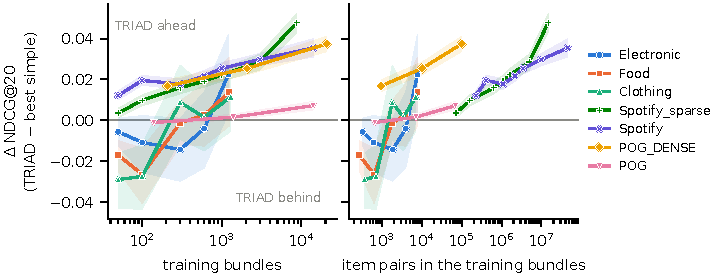
\includegraphics[width=.92\textwidth]{figs/fig3_budget.pdf}
\caption{TRIAD minus the best simple baseline (NDCG@20, clean test, 95\% interval) as training bundles are removed,
against the number of bundles (left) and the number of item pairs they contain (right). The simple baselines may use
the frequency prior (Section~\ref{sec:fair}); the best one is chosen on validation for every subset.}
\label{fig:budget}
\end{figure}

\begin{table}[t]
\centering
\caption{TRIAD minus the best simple baseline, NDCG@20 on clean test queries, by training-set size. Bold: interval
excludes zero and Holm-adjusted $p<.05$ within the domain. Pseudo: users' purchase histories as training bundles
(clean: histories that overlap test bundles removed).}
\label{tab:budget}
\setlength{\tabcolsep}{3.5pt}
\scriptsize
\begin{tabular}{lrrrrrrr}
\toprule
Dataset & full & 3,000 & 1,000 & 600 & 300 & 100 & 50\\
\midrule
Electronic & +.022 & & & $-$.004 & $-$.014 & $-$.011 & $-$.006\\
Food & +.014 & & & +.003 & $-$.001 & \textbf{$-$.027} & \textbf{$-$.017}\\
Clothing & +.011 & & & +.002 & +.009 & \textbf{$-$.028} & \textbf{$-$.029}\\
Spotify\_sparse & \textbf{+.048} & \textbf{+.029} & \textbf{+.022} & \textbf{+.019} & \textbf{+.016} & \textbf{+.010} & \textbf{+.004}\\
Spotify & \textbf{+.035} & \textbf{+.030} & \textbf{+.025} & \textbf{+.022} & \textbf{+.018} & \textbf{+.020} & \textbf{+.012}\\
\bottomrule
\end{tabular}

\medskip
\begin{tabular}{lrrrrr}
\toprule
Dataset & full & 10\% & 1\% & pseudo & pseudo, clean\\
\midrule
POG\_DENSE & \textbf{+.037} & \textbf{+.025} & \textbf{+.017} & \textbf{$-$.006} & \textbf{$-$.006}\\
POG & \textbf{+.007} & +.002 & \textbf{$-$.001} & \textbf{$-$.003} & \textbf{$-$.001}\\
\bottomrule
\end{tabular}
\end{table}

\paragraph{Playlists: TRIAD leads at every size.} On Spotify and Spotify\_sparse, TRIAD stays ahead down to 50
playlists (+.012 and +.004 NDCG@20), and all 28 tests reject after Holm (Table~\ref{tab:budget}). The lead shrinks
steadily as bundles are removed. Validation picks the baseline with the prior for 9 of the 14 subsets.

\paragraph{Outfits: ahead while enough real outfits remain.} On POG\_DENSE, TRIAD stays ahead with 10\% and 1\%
of the training outfits (+.025 and +.017). On POG it is +.002 with 10\% ($p=.06$) and slightly behind with 1\%
($-$.001). Trained instead on users' purchase histories, with no real outfits, it is slightly behind on both
($-$.001 to $-$.006), and all four of these differences are significant. On POG at 1\% and on POG's pseudo-bundles every
method scores below .004 NDCG@20.

\paragraph{Short e-commerce bundles: never significantly ahead, behind with 100 or fewer.} On Electronic, Food and
Clothing, TRIAD is not significantly different from the best simple baseline with the prior at any size from the full
1,200--1,300 bundles down to 300 ($-$.014 to +.022; none of the twelve tests rejects after Holm, and every interval on
Food and Clothing contains zero). With 100 and 50 bundles it is behind on all three, by .006--.029, significantly on Food and Clothing.
The baseline chosen there is label+ItemKNN+content with the prior. Before the baselines were given the prior, TRIAD
appeared ahead with all bundles and on Clothing with 600 and 300; that lead disappears once they get it.

\paragraph{The cause is overfitting.} Repeating the e-commerce subsets so that each epoch has as many gradient steps
as on the full data changes test NDCG@20 by at most .02; validation NDCG usually peaks after the first epoch and then
falls while the training loss keeps dropping (Food, 50 bundles: loss 5.86 to 0.44, validation NDCG .213 to .133).
Training improves on the untrained model in all nine cases, but with 100 or fewer bundles it overfits before it
catches up with the tuned simple scorer.

\paragraph{What predicts the outcome.} Bundle count alone does not: 50 playlists are enough, 100 product bundles are
not. A playlist holds about 1,700--3,300 item pairs, a product bundle about 6, so 50 playlists contain more pairs than
all e-commerce training sets (Fig.~\ref{fig:budget}, right). Pairs alone do not decide it either: POG\_DENSE at 1\%
(952 pairs) still favours TRIAD, as 34\% of its test targets occur in those bundles. With real bundles, TRIAD was
significantly behind only with under 1,000 pairs and at most 28\% of targets seen (Food and Clothing with 100 or 50
bundles, POG at 1\%), and significantly ahead only on outfits and playlists; this is an observation on seven datasets
rather than a tested rule.

\subsection{What TRIAD learns}
\label{sec:learned}

Every trained part of TRIAD is a function of a few interpretable inputs, so we can ask whether its trained values
mean something. For each part we compare what it learned with a quantity measured directly on validation data
(first 512 validation queries, seeds 0--2, never test). These readings describe what each part encodes; the
ablations (Section~\ref{sec:ablation}) test whether it helps. Table~\ref{tab:learned} gives the main values.

\begin{table}[t]
\centering
\caption{Learned values, mean of three seeds. Gate weights are averaged over validation queries. $\deltab_l$ is
evaluated for one of three seeds sharing the candidate's label, at the median label size. Music: labels and
$\deltab_l$ given as artist, album.}
\label{tab:learned}
\setlength{\tabcolsep}{4pt}
\small
\begin{tabular}{lrrrll}
\toprule
Dataset & $\theta$ & $\alpha$ & $\beta$ & Gate: content / labels / graph & $\deltab_l$\\
\midrule
Electronic & 1.87 & .06 & .13 & 1.89 / 0.63 / 4.94 & $+$0.21\\
Food & 1.63 & $-$.05 & $-$.06 & 2.13 / 0.87 / 4.05 & $+$1.00\\
Clothing & 1.68 & $-$.07 & $-$.18 & 2.58 / 1.06 / 5.72 & $+$1.27\\
POG\_DENSE & 4.84 & .41 & .36 & 5.68 / 0.45 / 2.96 & $\mathbf{-22.5}$\\
POG & 2.95 & .29 & .28 & 3.83 / 1.00 / 2.94 & $\mathbf{-6.17}$\\
Spotify\_sparse & 0.83 & $-$.07 & $-$.05 & 3.05 / 1.23, 1.27 / 0.82 & $+$1.88, $+$1.17\\
Spotify & 1.10 & .33 & $-$.30 & 3.08 / 0.92, 1.07 / 1.10 & $+$1.87, $+$1.20\\
\bottomrule
\end{tabular}
\end{table}

\begin{figure}[t]
\centering
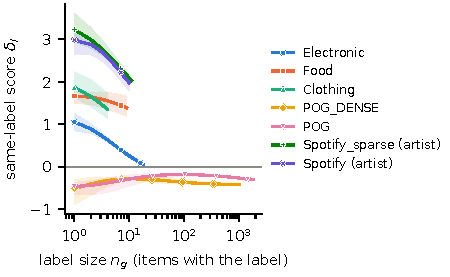
\includegraphics[width=.62\textwidth]{figs/fig4_delta.pdf}
\caption{The learned same-label score $\deltab_l$ for one shared seed ($m=1$) at the median query size, against the
size of the label (mean of three seeds, band: min to max). It is negative for fashion and positive for music and
e-commerce.}
\label{fig:delta}
\end{figure}

\paragraph{The sign of the label relation is learned.} $\deltab_l$ starts as a small random MLP with no fixed sign,
and after training it differs by domain (Fig.~\ref{fig:delta}). On POG and POG\_DENSE it is negative, more so for
large categories: an outfit rarely repeats a category. Weighted by the gate, a candidate in a seed's category loses
about 10 points on POG\_DENSE, more than any other term adds, and the label term's spread over each query's top 100
candidates is at most .003: every candidate that shares a seed's category is pushed out of the shortlist, so the
penalty works as a hard rule. On Spotify $\deltab_l$ is strongly positive for small artists, a sharp signal, and the
artist term moves the shortlist more than the album term (spread .66--1.00 against .35--.54). On e-commerce a shared
label gives a small bonus, which fades for large labels on Electronic and Clothing.

\begin{figure}[t]
\centering
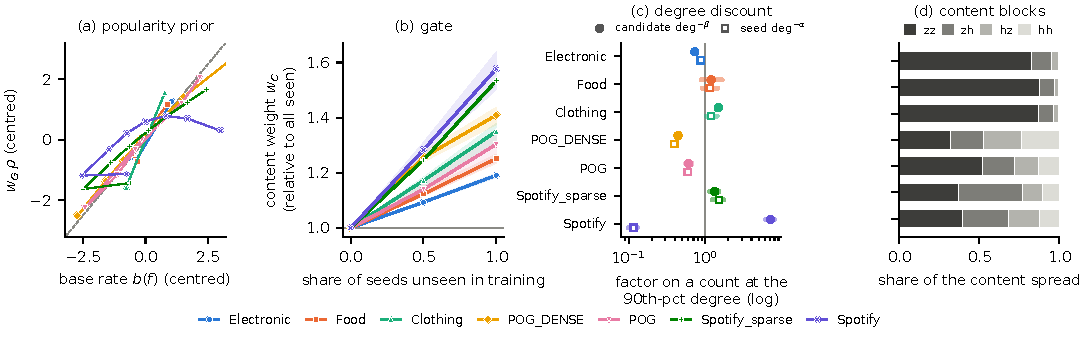
\includegraphics[width=\textwidth]{figs/fig5_params.pdf}
\caption{Reading the other parameters (validation queries, seeds 0--2). (a) The weighted popularity prior
$w_G\rho$ against the base rate $b(f)$ per frequency bin, both centred per dataset; the dashed line is equality.
(b) The gate's content weight as the share of seeds unseen in training goes from 0 to 1, other inputs at the median
query, relative to its value at 0 (band: min to max over seeds). (c) The factor $\deg^{-\beta}$ (candidate) and
$\deg^{-\alpha}$ (seed) on a count at the 90th-percentile degree (bars: range over seeds). (d) Share of the content
score's spread over the top 100 candidates due to each of its four blocks.}
\label{fig:params}
\end{figure}

\paragraph{$\rho$ learns the base rate of targets by popularity.} The loss is a softmax over the whole catalogue.
If the only score were a function of an item's training frequency $f$, the best such score would be the base rate
\[
b(f)=\log\frac{\text{share of targets with frequency } f}{\text{share of catalogue items with frequency } f},
\]
up to a constant, since a softmax ignores a shift of all scores. We group items into frequency bins (0, 1, 2, 3--4,
5--9, 10--19, 20--49, 50+, keeping bins with at least 20 items and 20 targets). The weighted prior $w_G\rho$ has the
shape of $b$ (Fig.~\ref{fig:params}a): the correlation over bins is .97--.99 on Electronic, .95--.97 on Food, .99 on
POG\_DENSE, 1.00 on POG and .93--.95 on Spotify\_sparse (Clothing has only two bins). On full Spotify it is .67--.71:
there $\beta\approx-.3$ already favours popular candidates and $\rho$ stays nearly flat.

\paragraph{Unseen items are more likely targets than items seen once.} On every dataset the base rate is higher at
$f=0$ than at $f=1$, by 1.4--2.3. The reason is how the released catalogues are built: they hold every item of every
split, so an item with $f=0$ is in the catalogue only because some validation or test bundle contains it. No test
label is needed to learn this: leave-one-out training produces the same situation from training bundles alone (an
item seen once has $f=0$ once its bundle is left out). $\rho$ learns the gap on e-commerce and POG (on Clothing it is
3.1, twice the base-rate gap), and little of it on Spotify (.04 and .29). Section~\ref{sec:fair} measures how much
of TRIAD's accuracy this accounts for and gives the simple baselines the same prior.

\paragraph{The gate moves weight to content when the seeds are unseen.} An unseen seed has no co-occurrence counts
and no partner history, so its evidence can only come from its features and labels. As the share of unseen seeds
goes from 0 to 1, the content weight rises on all seven datasets and in every seed, by 18--27\% on e-commerce,
24--44\% on POG and 50--64\% on Spotify (Fig.~\ref{fig:params}b). On Spotify both label weights rise as well (artist
0.73$\to$1.35, album 0.91$\to$2.00 on full Spotify) and the graph weight falls (1.13$\to$0.73). On Clothing and
POG\_DENSE the graph weight rises instead: with unseen seeds the graph term is mostly the prior $\rho$, which then
carries more weight. The content weight also grows with $|S|$ (POG: 5.3 at $|S|=2$, 12.8 at $|S|=20$); part of that
is rescaling, since the mean of more seed vectors is shorter, so we do not read it as meaning.

\paragraph{The degree exponents are readable on POG and Spotify.} A count $N_{sc}$ is multiplied by
$\deg_s^{-\alpha}\deg_c^{-\beta}$ (Fig.~\ref{fig:params}c). On POG, busy items are discounted on both sides
($\times$0.39--0.67 at the 90th-percentile degree), much like the normalization in RP3$\beta$. On full Spotify a hit
song as a seed says little about a playlist ($\times$0.10--0.13), but hits are likely candidates ($\times$6.1--7.9),
which is why $\rho$ can stay flat there. On the e-commerce sets degrees are small (about 10 at the 90th percentile),
so the exponents matter little; on Food and Spotify\_sparse they are small and change sign between seeds, so they are
not identified by the data and we do not read them.

\paragraph{Content: near title similarity on e-commerce, a new relation on POG and Spotify.} The content score is the
sum of four blocks, $C=\bar z^{\top}(A_z^{\top}B_z)z_c+\bar z^{\top}(A_z^{\top}B_h)h_c+\bar h^{\top}(A_h^{\top}B_z)z_c
+\bar h^{\top}(A_h^{\top}B_h)h_c$, called zz, zh, hz and hh. zz asks whether the seeds look like the candidate, zh
whether they look like the items the candidate is usually bundled with, a complement signal. On e-commerce zz gives
83--88\% of the spread (Fig.~\ref{fig:params}d), $A_z^{\top}B_z$ moves 11--27\% from its start and keeps over 97\% of
its mass in the first 64 dimensions, and the refined features stay close to the inputs (cosine .78--.92): content
stays close to ``similar title''. On POG\_DENSE the map is largely rebuilt (80--100\% change, 23--32\% of its mass
outside the first 64 dimensions) and all four blocks matter (21--32\% each): the model learns which looks go together,
not which look alike, which is what an outfit needs. On Spotify\_sparse ``sounds like the candidate's usual
neighbours'' (zh, 40\%) moves the shortlist as much as ``sounds like the candidate'' (zz, 37\%).

% =====================================================================================================================
\section{Conclusion}

We showed that bundle completion does not need a learned representation per item. TRIAD learns 41,368 shared
parameters that weight content similarity, label relations and co-occurrence for each query, and is trained with
statistics that never contain the training bundle itself. Under one protocol, with neural models rerun on identical
splits and features and simple baselines given the same information, it ranks missing items better than CLHE and
RaMen on every dataset, better than the best of thirteen tuned simple baselines on outfits and playlists, and as well
as the best of them on short e-commerce bundles. Its learned label relations, popularity prior, gate and degree
discounts are readable and, where the data identify them, match quantities measured directly on validation data.

\paragraph{Limitations.} On e-commerce TRIAD is not significantly ahead of a content and neighbourhood scorer that gets the
same frequency prior, and without its unseen-item bonus it is behind on Clothing. The released catalogues list the
items of every split; TRIAD's prior uses this, as can any model trained with a full-catalogue loss. With never-bundled
items added to the catalogue the learned bonus becomes a penalty and its gain vanishes, while TRIAD stays level with
the best simple baseline (Table~\ref{tab:catalogue}); this was checked on two e-commerce datasets with copied items,
not on a real store catalogue. The margins over the best simple baseline
are small on POG (+.007). Although TRIAD can score new items, features find unseen POG targets only at chance level,
so new items remain hard. On Dunnhumby grocery baskets, which are not bundles and are not part of our study, TRIAD is
level with the content+ItemKNN blend even without giving the blend the prior ($-$.003 [$-$.006, $-$.001] NDCG@20,
not separated after Holm). Scoring is linear in the catalogue size, so catalogues of millions of items would need a
candidate stage. Some baseline numbers (RaMen on POG and Spotify, Bundle-MLLM, CLHE on full Spotify) are published or
from one seed, not rerun.

\paragraph{Future work.} A natural next step is to start training from the tuned simple scorer and penalize moving
away from it, which may remove the small-data gap. Code will be released.

\begin{thebibliography}{99}\scriptsize
\bibitem{abdollahpouri2017} Abdollahpouri, H., Burke, R., Mobasher, B.: Controlling popularity bias in learning-to-rank recommendation. In: RecSys (2017)
\bibitem{bgn} Bai, J., Zhou, C., Song, J., Qu, X., An, W., Li, Z., Gao, J.: Personalized bundle list recommendation. In: WWW (2019)
\bibitem{bgcn} Chang, J., Gao, C., He, X., Jin, D., Li, Y.: Bundle recommendation with graph convolutional networks. In: SIGIR (2020)
\bibitem{spotify} Chen, C.W., Lamere, P., Schedl, M., Zamani, H.: RecSys Challenge 2018: Automatic music playlist continuation. In: RecSys (2018)
\bibitem{pog} Chen, W., et al.: POG: Personalized outfit generation for fashion recommendation at Alibaba iFashion. In: KDD (2019)
\bibitem{efron1993} Efron, B., Tibshirani, R.J.: An Introduction to the Bootstrap. Chapman \& Hall (1993)
\bibitem{dacrema} Ferrari Dacrema, M., Cremonesi, P., Jannach, D.: Are we really making much progress? A worrying analysis of recent neural recommendation approaches. In: RecSys (2019)
\bibitem{gartrell2017} Gartrell, M., Paquet, U., Koenigstein, N.: Low-rank factorization of determinantal point processes. In: AAAI (2017)
\bibitem{han2017} Han, X., Wu, Z., Jiang, Y.G., Davis, L.S.: Learning fashion compatibility with bidirectional LSTMs. In: ACM MM (2017)
\bibitem{lightgcn} He, X., Deng, K., Wang, X., Li, Y., Zhang, Y., Wang, M.: LightGCN: Simplifying and powering graph convolution network for recommendation. In: SIGIR (2020)
\bibitem{holm1979} Holm, S.: A simple sequentially rejective multiple test procedure. Scandinavian Journal of Statistics 6(2), 65--70 (1979)
\bibitem{hu2008} Hu, Y., Koren, Y., Volinsky, C.: Collaborative filtering for implicit feedback datasets. In: ICDM (2008)
\bibitem{kapoor2023} Kapoor, S., Narayanan, A.: Leakage and the reproducibility crisis in machine-learning-based science. Patterns 4(9) (2023)
\bibitem{krichene2020} Krichene, W., Rendle, S.: On sampled metrics for item recommendation. In: KDD (2020)
\bibitem{lightfm} Kula, M.: Metadata embeddings for user and item cold-start recommendations. In: CBRecSys Workshop at RecSys (2015)
\bibitem{settransformer} Lee, J., Lee, Y., Kim, J., Kosiorek, A., Choi, S., Teh, Y.W.: Set Transformer: A framework for attention-based permutation-invariant neural networks. In: ICML (2019)
\bibitem{blip} Li, J., Li, D., Xiong, C., Hoi, S.: BLIP: Bootstrapping language-image pre-training for unified vision-language understanding and generation. In: ICML (2022)
\bibitem{bundlemllm} Liu, X., Wu, J., Tao, Z., Ma, Y., Wei, Y., Chua, T.S.: Fine-tuning multimodal large language models for product bundling. In: KDD (2025)
\bibitem{adamw} Loshchilov, I., Hutter, F.: Decoupled weight decay regularization. In: ICLR (2019)
\bibitem{crosscbr} Ma, Y., He, Y., Zhang, A., Wang, X., Chua, T.S.: CrossCBR: Cross-view contrastive learning for bundle recommendation. In: KDD (2022)
\bibitem{clhe} Ma, Y., Liu, X., Wei, Y., Tao, Z., Wang, X., Chua, T.S.: Leveraging multimodal features and item-level user feedback for bundle construction. In: WSDM (2024)
\bibitem{mcauley} McAuley, J., Pandey, R., Leskovec, J.: Inferring networks of substitutable and complementary products. In: KDD (2015)
\bibitem{ramen} Nguyen, H.S., Nguyen, Q.H., Pham, D.H., Le, D.T., Le, H.Q., Sitkrongwong, P., Takasu, A., Mansoury, M.: RaMen: Multi-strategy multi-modal learning for bundle construction. In: ECAI (2025)
\bibitem{caro} Nguyen, L.H., Nguyen, H.S., Nguyen, C.V.T., Le, D.T., Takasu, A., Le, H.Q.: Dual-enhanced item representation for bundle construction via category-wise and cross-modality learning. In: SIGIR-AP (2025)
\bibitem{rp3beta} Paudel, B., Christoffel, F., Newell, C., Bernstein, A.: Updatable, accurate, diverse, and scalable recommendations for interactive applications. ACM TiiS 7(1) (2017)
\bibitem{sgfcf} Peng, S., Liu, X., Sugiyama, K., Mine, T.: How powerful is graph filtering for recommendation. In: KDD (2024)
\bibitem{bpr} Rendle, S., Freudenthaler, C., Gantner, Z., Schmidt-Thieme, L.: BPR: Bayesian personalized ranking from implicit feedback. In: UAI (2009)
\bibitem{rendle2020} Rendle, S., Krichene, W., Zhang, L., Anderson, J.: Neural collaborative filtering vs. matrix factorization revisited. In: RecSys (2020)
\bibitem{sarwar2001} Sarwar, B., Karypis, G., Konstan, J., Riedl, J.: Item-based collaborative filtering recommendation algorithms. In: WWW (2001)
\bibitem{gfcf} Shen, Y., Wu, Y., Zhang, Y., Shan, C., Zhang, J., Letaief, K.B., Li, D.: How powerful is graph convolution for recommendation? In: CIKM (2021)
\bibitem{smucker2007} Smucker, M.D., Allan, J., Carterette, B.: A comparison of statistical significance tests for information retrieval evaluation. In: CIKM (2007)
\bibitem{steck2019} Steck, H.: Embarrassingly shallow autoencoders for sparse data. In: WWW (2019)
\bibitem{bundlerec} Sun, Z., Feng, K., Yang, J., Fang, H., Qu, X., Ong, Y.S., Liu, W.: Revisiting bundle recommendation for intent-aware product bundling. ACM TORS 2(3) (2024)
\bibitem{adabundle} Sun, Z., Feng, K., Yang, J., Qu, X., Fang, H., Ong, Y.S., Liu, W.: Adaptive in-context learning with large language models for bundle generation. In: SIGIR (2024)
\bibitem{ddbc} Tu, T., Li, A., Ma, Y., Xu, S., Liu, X., Ma, H., Pang, L., Chua, T.S.: Discrete diffusion for bundle construction. In: ICLR (2026)
\bibitem{vasileva2018} Vasileva, M.I., Plummer, B.A., Dusad, K., Rajpal, S., Kumar, R., Forsyth, D.: Learning type-aware embeddings for fashion compatibility. In: ECCV (2018)
\bibitem{volkovs2018} Volkovs, M., Rai, H., Cheng, Z., Wu, G., Lu, Y., Sanner, S.: Two-stage model for automatic playlist continuation at scale. In: RecSys Challenge (2018)
\bibitem{dropoutnet} Volkovs, M., Yu, G., Poutanen, T.: DropoutNet: Addressing cold start in recommender systems. In: NeurIPS (2017)
\bibitem{clap} Wu, Y., Chen, K., Zhang, T., Hui, Y., Berg-Kirkpatrick, T., Dubnov, S.: Large-scale contrastive language-audio pretraining with feature fusion and keyword-to-caption augmentation. In: ICASSP (2023)
\bibitem{deepsets} Zaheer, M., Kottur, S., Ravanbakhsh, S., Poczos, B., Salakhutdinov, R., Smola, A.: Deep sets. In: NeurIPS (2017)
\end{thebibliography}
\end{document}
